\documentclass[main.tex]{subfiles}
\begin{document}

\href{https://www2.seas.gwu.edu/~simhaweb/quantum/modules/module3/module3.html}{Module 3: The Single Qubit}

\begin{enumerate}

\item[] \textbf{In-Class Exercise 1:} Suppose the qubit state is $|\psi\rangle=|+\rangle$ and the measurement basis is: $|w\rangle=\frac{\sqrt{3}}{2}|0\rangle-\frac{1}{2}|1\rangle$, and $\left|w^{\perp}\right\rangle=\frac{1}{2}|0\rangle+\frac{\sqrt{3}}{2}|1\rangle$. \textbf{Q.} What are the possible output vectors, and with what probabilities do they occur? Start by expressing $|+\rangle$ in the $|w\rangle$, $\left|w^{\perp}\right\rangle$ basis by computing the coefficients $\langle w \mid+\rangle,\left\langle w^{\perp} \mid+\right\rangle$. \textbf{A.} 
\begin{align*}
    |\psi\rangle                    & = \langle w \mid+\rangle |0\rangle +  \langle w^{\perp} \mid+\rangle | 1 \rangle\\
    \langle w \mid+\rangle          & = \frac{\sqrt{3}}{2}\langle 0 |- \frac{1}{2} \langle 1| \mid | + \rangle\\
                                    & = \left[ \begin{array}{ll} \frac{\sqrt{3}}{2} & -\frac{1}{2} \end{array} \right]
                                    \left[ \begin{array}{l} \frac{1}{\sqrt{2}} & \frac{1}{\sqrt{2}} \end{array} \right]\\
                                    & = \frac{\sqrt{3}-1}{2\sqrt{2}}\\
    \langle w^{\perp} \mid+\rangle  & = \frac{1}{2}\langle 0 | + \frac{\sqrt{3}}{2} \langle 1| \mid | + \rangle\\
                                    & = \left[ \begin{array}{ll} \frac{1}{2} & + \frac{\sqrt{3}}{2} \end{array} \right]
                                    \left[ \begin{array}{l} \frac{1}{\sqrt{2}} & \frac{1}{\sqrt{2}} \end{array} \right]\\
                                    & = \frac{\sqrt{3}+1}{2\sqrt{2}}\\
    |0\rangle                       & = \left| \frac{\sqrt{3}-1}{2\sqrt{2}} \right|^2 \tag{output vector}\\ 
                                    & =\frac{2-\sqrt{3}}{4} \tag{probability outcome}\\
    |1\rangle                       & = \left| \frac{\sqrt{3}+1}{2\sqrt{2}} \right|^2 \tag{output vector}\\
                                    & =\frac{2+\sqrt{3}}{4} \tag{probability outcome}
\end{align*}

\item[] \textbf{In-Class Exercise 2:} \textbf{Q.} What does the $X$ gate do to the state $|\psi\rangle=\alpha|0\rangle+\beta|1\rangle$? \textbf{A.} 
\begin{align*}
    X |\psi\rangle  & = \alpha X |0\rangle + \beta X|1\rangle\\
                    & =  \alpha \left[\begin{array}{ll} 0 & 1 \\ 1 & 0 \end{array}\right] \left[\begin{array}{l} 1 \\ 0 \end{array} \right]
                    + \beta \left[\begin{array}{ll} 0 & 1 \\ 1 & 0 \end{array}\right] \left[\begin{array}{l} 0 \\ 1 \end{array} \right]\\
                    & = \beta |0\rangle + \alpha |1\rangle\\
\end{align*}

\item[] \textbf{In-Class Exercise 3:} \textbf{Q.} Derive the above result that applies $H$ to $|\psi\rangle=\alpha|0\rangle+\beta|1\rangle$. Also show that $H|\psi\rangle=\alpha|+\rangle+\beta|-\rangle$. \textbf{A.}
\begin{align*}
    | \psi \rangle      & = H \left( \alpha | 0 \rangle + \beta | 1 \rangle \right) \\
                        & = \left[\begin{array}{ll} \frac{1}{\sqrt{2}} & \frac{1}{\sqrt{2}} \\ \frac{1}{\sqrt{2}} & -\frac{1}{\sqrt{2}} \end{array} \right] 
                        \left[\begin{array}{l} \alpha \\ \beta \end{array} \right]\\
                        & =  \left[\begin{array}{l} \frac{\alpha + \beta}{\sqrt{2}} \\ \frac{\alpha - \beta}{\sqrt{2}} \end{array} \right] \\
                        & = \frac{\alpha+\beta}{\sqrt{2}}|0\rangle+\frac{\alpha-\beta}{\sqrt{2}}|1\rangle \\
    H | \psi \rangle    & = \alpha H | 0 \rangle + \beta H | 1 \rangle \\
                        & =  \alpha \left[\begin{array}{ll} \frac{1}{\sqrt{2}} & \frac{1}{\sqrt{2}} \\ \frac{1}{\sqrt{2}} & -\frac{1}{\sqrt{2}} \end{array}\right] \left[\begin{array}{l} 1 \\ 0 \end{array} \right]
                        + \beta \left[\begin{array}{ll} \frac{1}{\sqrt{2}} & \frac{1}{\sqrt{2}} \\ \frac{1}{\sqrt{2}} & -\frac{1}{\sqrt{2}} \end{array}\right] \left[\begin{array}{l} 0 \\ 1 \end{array} \right]\\
                        & =  \alpha \left[\begin{array}{l} \frac{1}{\sqrt{2}} \\ \frac{1}{\sqrt{2}} \end{array} \right]
                        + \beta \left[\begin{array}{l} \frac{1}{\sqrt{2}} \\ -\frac{1}{\sqrt{2}} \end{array} \right]\\
                        & = \alpha | + \rangle + \beta | - \rangle
\end{align*}

\item[] \textbf{In-Class Exercise 4:} Consider the two circuits below, each given the same input.

    \begin{enumerate}
        \item[1.] \textbf{Q.} Write down the possible states of the outputs. \textbf{A.}
            \begin{align*}
                \text{Circuit 1 states } & = |0\rangle \text{ and } |1\rangle\\
                \text{Circuit 2 states } & = |+\rangle \text{ and } |-\rangle
            \end{align*}
        \item[2.] \textbf{Q.} Calculate the probabilities associated with each output state. \textbf{A.}
            \begin{align*}
                |\psi\rangle                    & = a|0\rangle+\beta|1\rangle\\
                |\psi\rangle                    & = H \left( \alpha | 0 \rangle + \beta | 1 \rangle \right) \\
                                                & = \frac{\alpha+\beta}{\sqrt{2}}|0\rangle+\frac{\alpha-\beta}{\sqrt{2}}|1\rangle \\
                |0\rangle \text{ probability }  & = \left(\frac{\alpha+\beta}{\sqrt{2}}\right)^{2}\\
                |1\rangle \text{ probability }  & = \left(\frac{\alpha-\beta}{\sqrt{2}}\right)^{2}\\
                H | \psi \rangle                & = \alpha H | 0 \rangle + \beta H | 1 \rangle \\
                                                & = \alpha | + \rangle + \beta | - \rangle\\
                |+\rangle \text{ probability }  & = \alpha^2\\
                |-\rangle \text{ probability }  & = \beta^2\\
                |\psi\rangle                    & = H \left( \alpha | + \rangle + \beta | - \rangle \right)\\
                                                & = \left[\begin{array}{ll} \frac{1}{\sqrt{2}} & \frac{1}{\sqrt{2}} \\ \frac{1}{\sqrt{2}} & -\frac{1}{\sqrt{2}} \end{array}\right] \left[\begin{array}{l} \frac{\alpha + \beta}{\sqrt{2}} \\ \frac{\alpha - \beta}{\sqrt{2}} \end{array} \right]\\
                                                & = \left[\begin{array}{l} \alpha \\ \beta \end{array} \right]
            \end{align*}
    \end{enumerate}

\item[] \textbf{In-Class Exercise 5:} \textbf{Q.} Considering Figure \ref{fig:e05polarizer}, what percentage of $|1\rangle$ photons arriving on the left reach the output? Work through your probability calculations as shown above. \textbf{A.}

    \begin{figure}
      \centering
      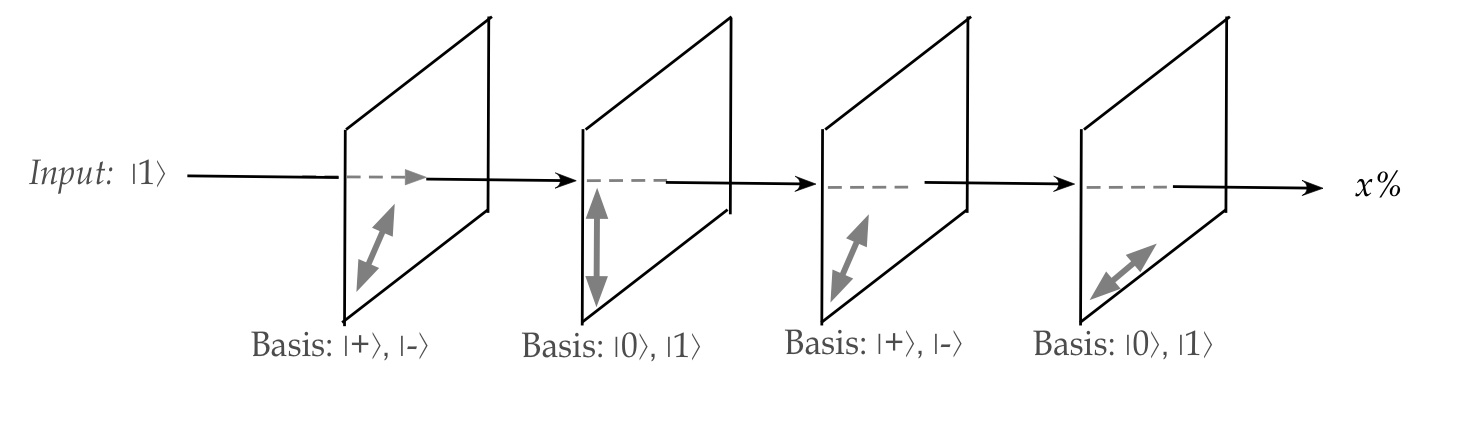
\includegraphics[width=5in]{modules/figs/m03/e05polarizer.png}
      \caption{Polarizer}
      \label{fig:e05polarizer}
    \end{figure}

    \begin{align*}
        |1\rangle                           & = \tag{input state}\\
                                            & = \frac{1}{\sqrt{2}}|+\rangle-\frac{1}{\sqrt{2}}|-\rangle \tag{device basis}\\
        |+\rangle                           & = \frac{1}{\sqrt{2}}|0\rangle+\frac{1}{\sqrt{2}}|1\rangle 
                                            = \text { pass through, polarized at } 45^{\circ} \tag {first polariser} \\
        |-\rangle                           & = \frac{1}{\sqrt{2}}|0\rangle-\frac{1}{\sqrt{2}}|1\rangle 
                                            = \text { absorb } \tag{first polariser}\\
        \left|\frac{1}{\sqrt{2}}\right|^{2} & = \frac{1}{2} \tag {probability of passing through}\\
        |+\rangle                           & = \tag{current state}\\
                                            & = \frac{1}{\sqrt{2}}|0\rangle+\frac{1}{\sqrt{2}}|1\rangle \tag{device basis}\\
        |0\rangle                           & = \text{ pass through, vertically polarized } \tag{second polariser}\\
        |1\rangle                           & = \text{ absorb } \tag{second polariser}\\
        \left|\frac{1}{\sqrt{2}}\right|^{2} & = \frac{1}{2} \tag {probability of passing through}\\
        |0\rangle                           & = \tag{current state}\\
                                            & = \frac{1}{\sqrt{2}}|+\rangle+\frac{1}{\sqrt{2}}|-\rangle \tag{device basis}\\
        |+\rangle                           & = \frac{1}{\sqrt{2}}|0\rangle+\frac{1}{\sqrt{2}}|1\rangle 
                                            = \text { pass through, polarized at } 45^{\circ} \tag {third polariser} \\
        |-\rangle                           & = \frac{1}{\sqrt{2}}|0\rangle-\frac{1}{\sqrt{2}}|1\rangle 
                                            = \text { absorb } \tag{third polariser}\\
        \left|\frac{1}{\sqrt{2}}\right|^{2} & = \frac{1}{2} \tag {probability of passing through}\\
        |+\rangle                           & = \tag{current state}\\
                                            & = \frac{1}{\sqrt{2}}|0\rangle+\frac{1}{\sqrt{2}}|1\rangle \tag{device basis}\\
        |0\rangle                           & = \text{ absorb  } \tag{fourth polariser}\\
        |1\rangle                           & = \text{ pass through, horizontally polarized } \tag{fourth polariser}\\
        \left|\frac{1}{\sqrt{2}}\right|^{2} & = \frac{1}{2} \tag {probability of passing through}\\
        |1\rangle                           & = \tag{current state}\\
        \left(\frac{1}{2}\right)^4          & = \frac{1}{16} = 6.25\% \tag{percentage of $|1\rangle$ photons at output}
    \end{align*}

\item[] \textbf{In-Class Exercise 6:}

    \begin{enumerate}
        \item[1.] \textbf{Q.} What would go wrong if the S-H strings were exchanged before Bob performs qubit measurements? \textbf{A.} In BB84 Step 5 Bob measures Alice's qubits using two bases, depending on his "S-H" string, and after which he will have a key bit-string aligned with his S-H string. If Bob exchanges his S-H string with Alice's in step 6 prior to calculating his key in step 5, then in Case 2 he will be unable to throw out bits where they differed in S-H because he will not know the original basis Alice used when encoding each original bit, resulting in a probability of inferring the correct bit of 0.5.
        
        \item[2.] \textbf{Q.} Write out the details of Case 2(B) above, explaining the details of measurement and probabilities. \textbf{A.} If Alice sends a 0 bit as an $|0\rangle$ qubit using the $\mathbf{S}$ basis and Bob uses the $\mathbf{H}$ basis to measure $|0\rangle = \frac{1}{\sqrt{2}}|+\rangle + \frac{1}{\sqrt{2}}|-\rangle$, $\alpha = \frac{1}{\sqrt{2}}$, with the probability Bob gets $|+\rangle = |\alpha|^2 = \frac{1}{2} = 0.5$, and infers $0$ with probability $0.5$. If Alice sends a 1 bit as an $|1\rangle$ qubit using the $\mathbf{S}$ basis and Bob uses the $\mathbf{H}$ basis to measure $|1\rangle = \frac{1}{\sqrt{2}}|+\rangle - \frac{1}{\sqrt{2}}|-\rangle$, $\beta = -\frac{1}{\sqrt{2}}$, with the probability Bob gets $|-\rangle = |\beta|^2 = \frac{1}{2} = 0.5$, and infers $1$ with probability $0.5$. 
    \end{enumerate}

\item[] \textbf{In-Class Exercise 7:} \textbf{Q.} Show that with $a,|\psi\rangle$ and $\left|\psi^{\prime}\right\rangle$ defined above, \textbf{A.}

    \begin{enumerate}
        \item[1.] $|a|^{2}=1$
        \begin{align*}
            a       & = \frac{2}{\sqrt{6}}-i \frac{\sqrt{2}}{\sqrt{6}}\\
            |a|^2   & = |\frac{2}{\sqrt{6}}-i \frac{\sqrt{2}}{\sqrt{6}}|^2\\
                    & = \frac{4}{6} + \frac{2}{6}\\
                    & = 1
        \end{align*}
        \item[2.] $\left|\psi^{\prime}\right\rangle=a|\psi\rangle$
        \begin{align*}
            |\psi\rangle                        & = \frac{\sqrt{2}}{\sqrt{3}}|0\rangle+\frac{1}{\sqrt{3}}|1\rangle\\
            a                                   & = \frac{2}{\sqrt{6}}-i \frac{\sqrt{2}}{\sqrt{6}}\\
            a |\psi\rangle                      & = \left(\frac{2\sqrt{2}-2i}{3\sqrt{2}}\right)|0\rangle
                                                +\left(\frac{2-i\sqrt{2}}{3\sqrt{2}}\right)|1\rangle\\
                                                & = \left(\frac{2-\sqrt{2}i}{3}\right)|0\rangle
                                                +\left(\frac{\sqrt{2}-i}{3}\right)|1\rangle\\
                                                & = \left|\psi^{\prime}\right\rangle
        \end{align*}
        \end{enumerate}
        
\textbf{Q.} Then, show that $|\psi\rangle$ and $a|\psi\rangle$ are indistinguishable no matter what basis is used, as long as $|a|^{2}=1$. (Hint: express the standard-basis vectors in terms of an arbitrary basis.) \textbf{A.}

    \begin{align*}
        |\psi\rangle                        & = \frac{\sqrt{2}}{\sqrt{3}}|0\rangle+\frac{1}{\sqrt{3}}|1\rangle\\
                                            & = \frac{\sqrt{2}}{\sqrt{3}}\left(\frac{1}{\sqrt{2}}|+\rangle+\frac{1}{\sqrt{2}}|-\rangle\right)
                                            +\frac{1}{\sqrt{3}}\left(\frac{1}{\sqrt{2}}|+\rangle-\frac{1}{\sqrt{2}}|-\rangle\right)\\
                                            & = \frac{\sqrt{2}+1}{\sqrt{6}}|+\rangle+\frac{\sqrt{2}-1}{\sqrt{6}}|-\rangle\\
        a                                   & = \frac{2}{\sqrt{6}}-i \frac{\sqrt{2}}{\sqrt{6}}\\
        a |\psi\rangle                      & = \frac{2\sqrt{2}+2-i\left(2+\sqrt{2}\right)}{6}|+\rangle
                                            +\frac{2\sqrt{2}-2-i\left(2-\sqrt{2}\right)}{6}|-\rangle\\
                                            & = \left(\frac{2+\sqrt{2}-i\left(\sqrt{2}+1\right)}{3\sqrt{2}}\right)|+\rangle
                                            +\left(\frac{2-\sqrt{2}-i\left(\sqrt{2}-1\right)}{3\sqrt{2}}\right)|-\rangle\\
        \left|\psi^{\prime}\right\rangle    & = \left(\frac{2-\sqrt{2} i}{3}\right)|0\rangle
                                            +\left(\frac{\sqrt{2}-i}{3}\right)|1\rangle\\
                                            & = \left(\frac{2-\sqrt{2} i}{3}\right)\left(\frac{1}{\sqrt{2}}|+\rangle+\frac{1}{\sqrt{2}}|-\rangle\right)
                                            +\left(\frac{\sqrt{2}-i}{3}\right)\left(\frac{1}{\sqrt{2}}|+\rangle-\frac{1}{\sqrt{2}}|-\rangle\right)\\
                                            & = \left(\frac{2+\sqrt{2}-i\left(\sqrt{2}+1\right)}{3\sqrt{2}}\right)|+\rangle
                                            +\left(\frac{2-\sqrt{2}-i\left(\sqrt{2}-1\right)}{3\sqrt{2}}\right)|-\rangle\\
    \end{align*}
        
\item[] \textbf{In-Class Exercise 8:} \textbf{Q.} Write down the two projector matrices $P_{v}, P_{v^{\perp}}$ for the general 2D basis $|v\rangle=a|0\rangle+b|1\rangle$, and $\left|v^{\perp}\right\rangle=b^{*}|0\rangle-a^{*}|1\rangle$ and check your calculations by showing $P_{v} P_{v^{\perp}}=0$. \textbf{A.}

    \begin{align*}
        P_{v}               & = |v\rangle\langle v| \\
                            & = \left[\begin{array}{l} a \\ b \end{array}\right] \left[\begin{array}{ll} a^{*} & b^{*} \end{array}\right]\\
                            & = \left[\begin{array}{ll} a a^{*} & a b^{*} \\ b a^{*} & b b^{*} \end{array}\right]\\
        P_{v^{\perp}}       & = \left|v^{\perp}\right\rangle \left\langle v^{\perp}\right|\\
                            & = \left[\begin{array}{l} b^{*} \\ -a^{*} \end{array}\right] \left[\begin{array}{ll} b & -a \end{array}\right]\\
                            & = \left[\begin{array}{ll} b^{*} b & -b^{*} a  \\ -a^{*} b & a^{*} a \end{array}\right]\\
        P_{v}P_{v^{\perp}}  & = \left[\begin{array}{ll} a a^{*} & a b^{*} \\ b a^{*} & b b^{*} \end{array}\right]
                            \left[\begin{array}{ll} b^{*} b & -b^{*} a \\ -a^{*} b & a^{*} a \end{array}\right]\\
                            & = a a^{*} b^{*} b - a b^{*} a^{*} b \\
                            & = 0
    \end{align*}

\item[] \textbf{In-Class Exercise 9:} \textbf{Q.} Suppose the qubit state is $|\psi\rangle=|+\rangle$ and the measurement basis is: $|w\rangle=\frac{\sqrt{3}}{2}|0\rangle-\frac{1}{2}|1\rangle$, and $\left|w^{\perp}\right\rangle=\frac{1}{2}|0\rangle+\frac{\sqrt{3}}{2}|1\rangle$. Apply the projective measurement approach: 

    \begin{enumerate}
        \item[1.] \textbf{Q.} Compute the projectors $P_{w}, P_{w^{\perp}}$.
        \begin{align*}
            
        \end{align*}
        \item[2.] \textbf{Q.} Apply the three steps, simplifying where possible.
    \end{enumerate}
    
     \textbf{Q.} Confirm that you get the same results as in Exercise 1.

\item[] \textbf{In-Class Exercise 10:}  \textbf{Q.} Use the projector matrices for the basis and the numbers $\gamma_{1}=3, \gamma_{2}=5$ to construct the Hermitian. Then show that these are the eigenvalues with $k t+,|-\rangle$ as eigenvectors.  \textbf{A.}

\item[] \textbf{In-Class Exercise 11:}  \textbf{Q.} Suppose the qubit state is $|\psi\rangle=|+\rangle$ and the measurement basis is: $|w\rangle=\frac{\sqrt{3}}{2}|0\rangle-\frac{1}{2}|1\rangle$, and $\left|w^{\perp}\right\rangle=\frac{1}{2}|0\rangle+\frac{\sqrt{3}}{2}|1\rangle .$ Compute $\left\langle+\left|P_{w}\right|+\right\rangle$ and $\left\langle+\left|P_{w^{\perp}}\right|+\right\rangle .$  \textbf{A.}

\item[] \textbf{In-Class Exercise 12:}  \textbf{Q.} Show that the Hadamard matrix can be written as $H=\frac{1}{\sqrt{2}} \backslash$ parenl $|0\rangle\langle 0|+| 0\rangle\langle 1|+| 1\rangle\langle 0|-| 1\rangle\langle 1|$ and then apply it to $|\psi\rangle=\alpha|0\rangle+\beta|1\rangle .$  \textbf{A.}

finish

\end{enumerate}
\end{document}